\chapter{TINJAUAN PUSTAKA DAN DASAR TEORI}
\label{chap:tinjauanpustaka}

% Ubah bagian-bagian berikut dengan isi dari tinjauan pustaka

Untuk mendapatkan informasi secara teoritis. Dilakukan sebuah pencarian untuk memberikan pemahaman yang cukup dalam melakukan pengerjaan Tugas Akhir ini. Berikut ini merupakan tinjauan pustaka yang menjadi landasan pemahaman.

\section{Kerangka dan Rotor Helikopter}
\label{sec:strukturheli}

Helikopter merupakan bentuk aplikasi dari prinsip-prinsip dasar fundametal hukum fisika, dimulai dari hukum pertama, kedua dan ketiga Newton, prinsip Bernoulli, konservasi energi dan aerodinamika. Keempat hukum dasar tersebut adalah sedikit dari prinsip fisika yang menjadi teori fundamental dari helikopter. Kompleksitas dibalik mengapa helikopter bisa terbang dapat dimengerti oleh pilot pemula sekalipun melalui pemahaman yang mendalam terhadap teori fisika yang berada pada helikopter\cite{wagtendonk2006principles}.

Helikopter memiliki banyak komponen (gambar \ref{fig:komponenheli}), dimulai dari sistem transmisi yang dilakukan oleh mesin menuju rotor utama, rotor pada ekor, dan komponen lain yang bergantung pada propulsi mesin. Bagian dari transmisi pada helikopter terdiri dari gigi rotor utama, poros penggerak, unit \textit{freewheeling}, rem rotor dan roda gigi rotor pada ekor  \cite{wagtendonk2006principles}.

\begin{figure}[H]
	\centering
	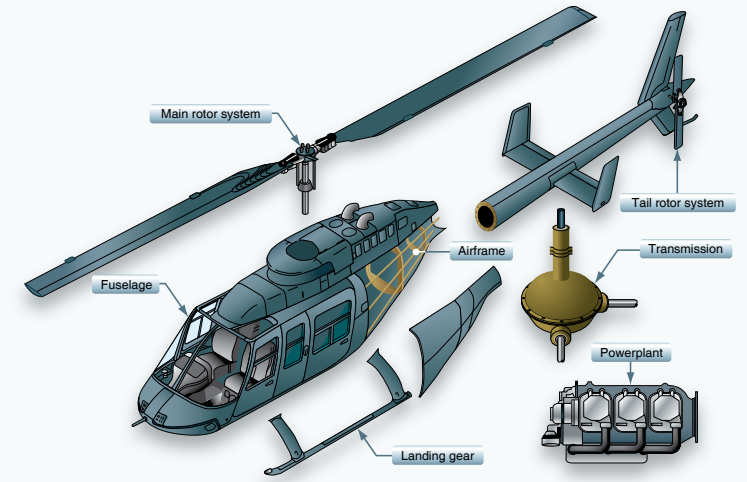
\includegraphics[width=0.8\linewidth]{gambar/komponenheli.png}
	\caption{Komponen helikopter secara umum \cite{handbook}.}
	\label{fig:komponenheli}
\end{figure}

\textit{Fuselage} badan helikopter merupakan bagian inti luar dari rangka yang menampung kabin berisi kru, penumpang, dan kargo. Kabin helikopter memiliki susunan tempat duduk yang berbeda-beda. Selain itu, badan helikopter juga berfungsi untuk memberikan ruang pada mesin, transmisi, avionik, kontrol penerbangan sumber power pada helikopter. Untuk sistem transmisi helikopter, mesin pada gigi rotor utama akan membuat poros rotor berputar. Ketika rotor berputar pada rpm mesin, kecepatan ujung rotor akan lebih cepat daripada kecepatan suara, kekuatan pada rotor harus ditingkatkan dan kelembaman dari giroskop akan menjadi sangat ekstrim. Terdapat bagian yang dinamakan \textit{clutch} (kopling) (gambar \ref{fig:clutch}) yaitu bagian yang terintegrasi dengan sistem transmisi. Bagian ini memungkinkan pilot untuk dapat mengatur kontak antara mesin dan poros penggerak \cite{wagtendonk2006principles}.

\begin{figure}[H]
	\begin{subfigure}{0.3\textwidth}
	\centering
	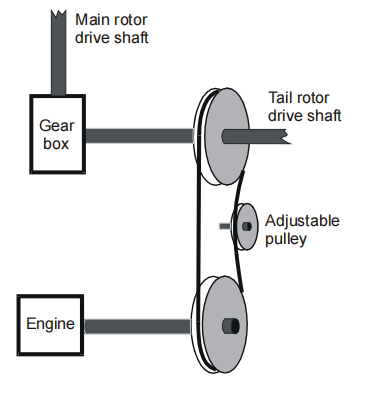
\includegraphics[width=\linewidth]{gambar/belt-driven_clutch.png}
	\caption{}
	\label{fig:belt-driven_clutch}
	\end{subfigure}
\centering
	\begin{subfigure}{0.3\textwidth}
	\centering
	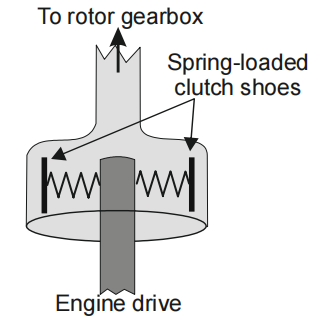
\includegraphics[width=\linewidth]{gambar/centrifugal_clutch.png}
	\caption{}
	\label{fig:centrifugal_clutch}
\end{subfigure}
	\caption{(a) Pengaturan kopling (\textit{clutch}) yang dihubungkan menggunakan sabuk. (b) Prinsip kopling sentrifugal \cite{handbook}.}
	\label{fig:clutch}
\end{figure}

Untuk mengatur pergerakannya, terdapat bagian komponen yang disebut dengan \textit{swashplate}, dapat dilihat pada gambar \ref{fig:swashplate}. Komponen ini dapat mengatur orientasi rotor utama dan jumlah gaya dorong rotor yang dihasilkan. Bearing (bola kecil) pada bagian \textit{swashplate} disesuaikan antara kedua piringan rotor yang bergerak. Sehingga gerakan piringan yang digerakkan oleh pilot akan berpindah ke rotor \cite{wagtendonk2006principles}.

\begin{figure}[H]
	\centering
	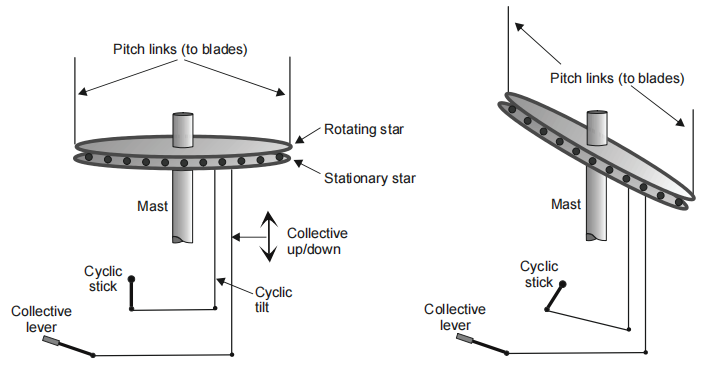
\includegraphics[width=0.7\linewidth]{gambar/swashplate.png}
	\caption{Mekanisme kontrol pada gerakan rotor utama \cite{handbook}.}
	\label{fig:swashplate}
\end{figure}
Sistem \textit{fully articulated rotor} mempunyai kemampuan pada rotornya untuk melakukan \textit{lead/lag} (gerakan kedepan dan belakang), \textit{flap} (gerakan atas dan bawah) dan \textit{feather} (berotasi pada sumbu radial) untuk merubah gaya angkat \cite{handbook} yang dapat dilihat pada gambar \ref{fig:fullyarticulated}.

\begin{figure}[H]
	\centering
	\begin{subfigure}{0.17\textwidth}
		\centering
		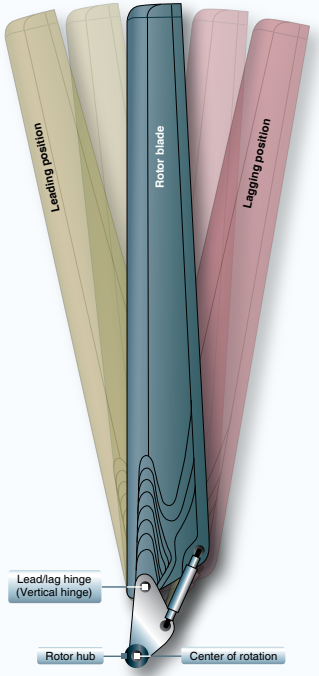
\includegraphics[width=\linewidth]{gambar/lead-lag.png}
		\caption{}
		\label{fig:lead/lag}
	\end{subfigure}
	\centering
	\begin{subfigure}{0.4\textwidth}
		\centering
		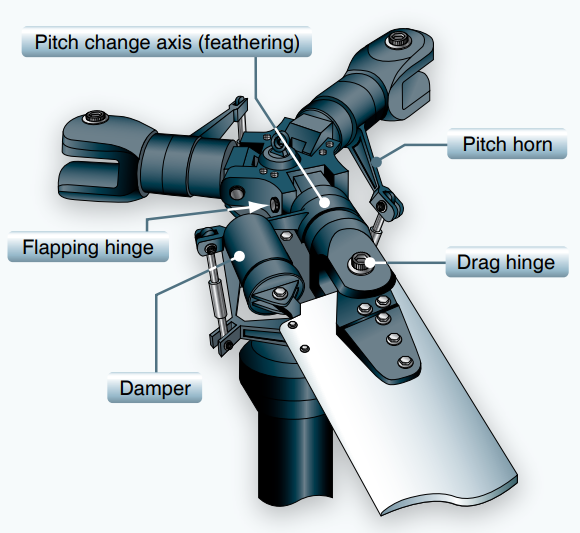
\includegraphics[width=\linewidth]{gambar/feather_flap.png}
		\caption{}
		\label{fig:featherflap}
	\end{subfigure}
	\caption{(a) Komponen \textit{lead/lag} membuat rotor dapat bergerak kedepan dan belakang pada bidangnya. (b) Komponen \textit{feather} dan \textit{flap} untuk gerakan rotasi pada arah radial serta bergerak atas bawah \cite{handbook}.}
	\label{fig:fullyarticulated}
\end{figure}

\begin{figure}[H]
	\centering
	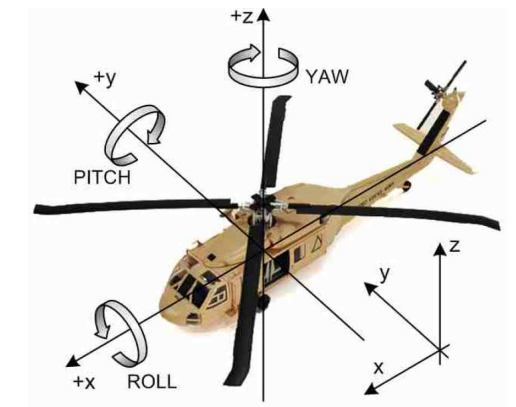
\includegraphics[width=0.68\linewidth]{gambar/roll-pitch-yaw.png}
	\caption{Orientasi arah helikopter \cite{Jhwang}.}
	\label{fig:orientasiheli}
\end{figure}

Saat rotor berputar, bilah pada rotor merespon \textit{input} dari kontrol untuk mengendalikan helikopter. Pusat daya angkat pada rotor akan bergerak karena respon yang diberikan \textit{input}, sehingga dapat menghasilkan gerakan \textit{pitch}, \textit{roll}, dan \textit{yaw} seperti yang dapat dilihat pada gambar \ref{fig:orientasiheli}. Arah gaya angkat ini bergantung pada \textit{input pitch} dan \textit{roll} dari pilot. Oleh karena itu, sudut \textit{feathering} pada setiap bilah akan berbanding lurus dengan gaya angkatnya, yaitu berubah saat berputar dengan rotor, gerakan ini disebut dengan \textit{cyclic control} \cite{handbook}.

Saat daya angkat meningkat, \textit{flapping hinge} akan mengayun ke arah atas tanpa kehilangan keseimbangan dengan gaya sentrifugal dari berat bilah rotor, dimana gaya tersebut akan tetap mempertahankan gerakannya untuk tetap pada bidang horizontal. Gaya sentrifugal pada dasarnya memiliki nilai yang konstan, namun gaya ayunan dipengaruhi oleh kecepatan naik, maju, dan berat helikopter. Sehingga saat bilah rotor berayun, pusat gravitasinya ikut berubah \cite{handbook}.

\section{\textit{Ground Resonance}}
\label{sec:groundresonance}

\textit{Ground resonance} adalah getaran dengan amplitudo besar yang disebabkan oleh osilasi pada helikopter yang sedang berada di tanah. Tanda awal resonansi ditandai dengan gerakan perlahan pada badan helikopter. Jika dibiarkan secara terus menerus, makana intensitas getaran akan semakin besar dan meningkat dengan cepat, sehingga berpotensi menyebabkan kerusakan pada pesawat \cite{wagtendonk2006principles}.

Fenomena \textit{ground resonance} merupakan getaran mekanis yang timbul secara otomatis dan terjadi pada sistem \textit{fully articulated rotor}. Engsel pada helikopter dengan sistem ini memberikan kebebasan pada masing-masing bilah rotor untuk bergerak dalam bidang rotasi rotor. Gerakan yang berlawanan dengan arah rotasi rotor disebut \textit{lagging}, sedangkan gerakan yang searah dengan rotasi disebut dengan \textit{leading}. Masing-masing bilah rotor memungkinkan untuk melakukan \textit{leading} atau \textit{lagging} untuk mengkompensasi perubahan drag yang terjadi ketika bilah rotor berayun karena adanya asimetri daya angkat dalam gerakan maju helikopter \cite{Eckert2007AnalyticalAA}.

Parameter yang penting terkait fenomena \textit{ground resonance} adalah frekuensi dan redaman pada mode \textit{lag} rotor, frekuensi dan redaman pada \textit{fuselage}, dan \textit{mode shape} pada \textit{fuselage}. Sehingga, identifikasi terhadap beban aerodinamik tidaklah menjadi penting. Karena dalam kondisi di ruang vakum pun \textit{ground resonance} juga tetap dapat terjadi pada helikopter \cite{bramwell2001bramwell}.

\begin{figure}[H]
	\centering
	\begin{subfigure}{0.4\textwidth}
		\centering
		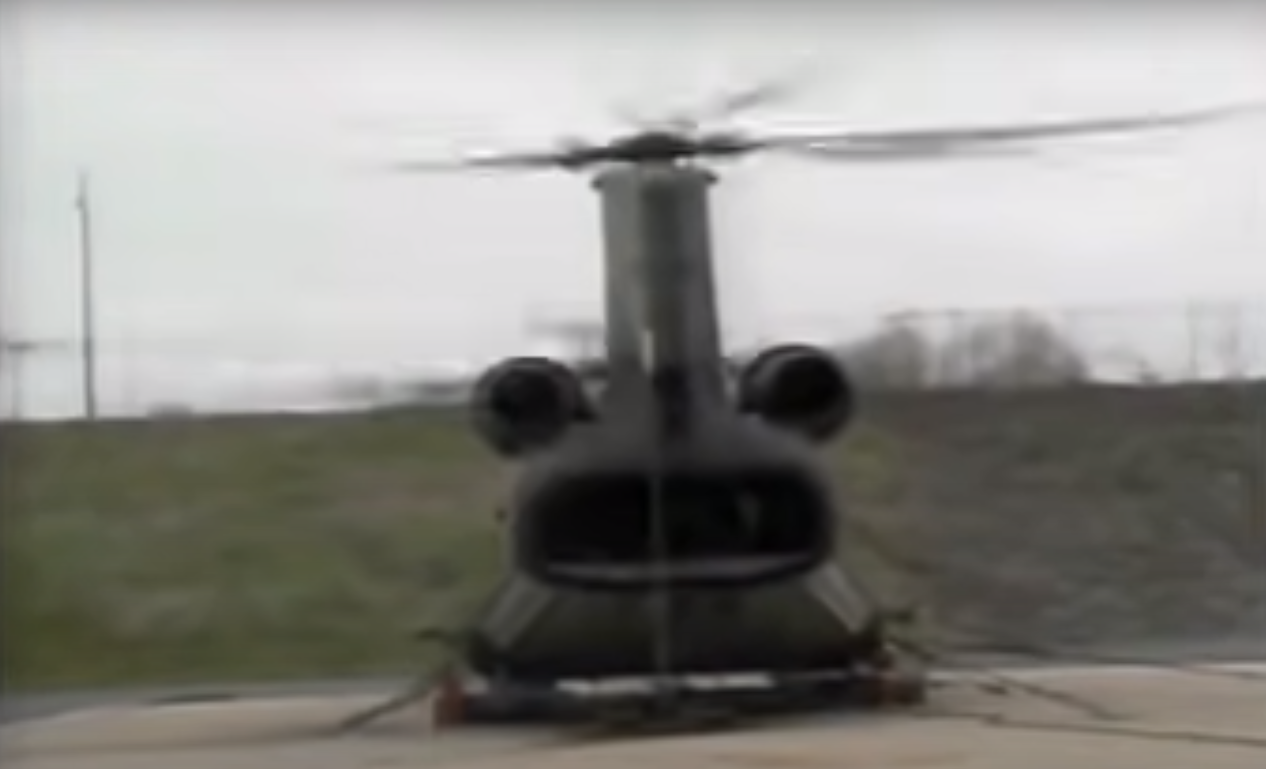
\includegraphics[width=\linewidth]{gambar/gr_1.png}
		\caption{}
		\label{fig:gr_1}
	\end{subfigure}
	\centering
	\begin{subfigure}{0.4\textwidth}
		\centering
		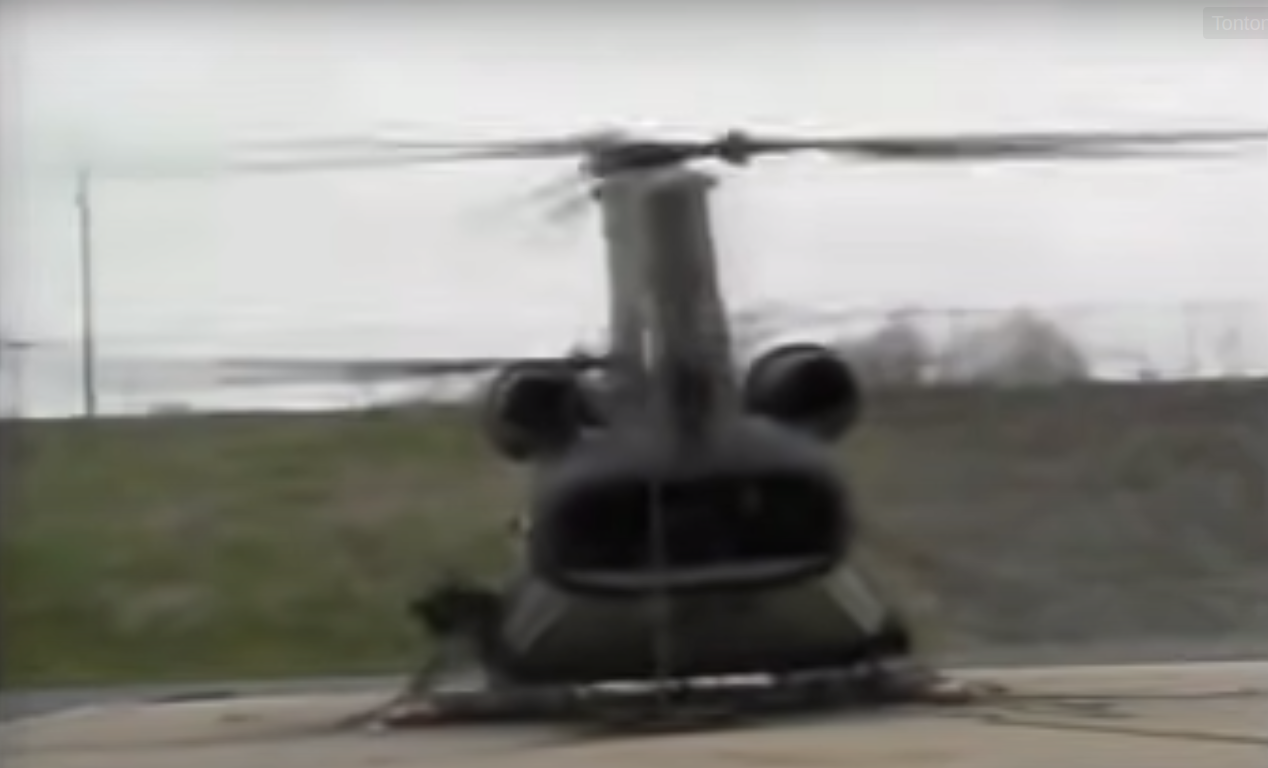
\includegraphics[width=\linewidth]{gambar/gr_2.png}
		\caption{}
		\label{fig:gr_2}
	\end{subfigure}
\\
	\centering
	\begin{subfigure}{0.4\textwidth}
		\centering
		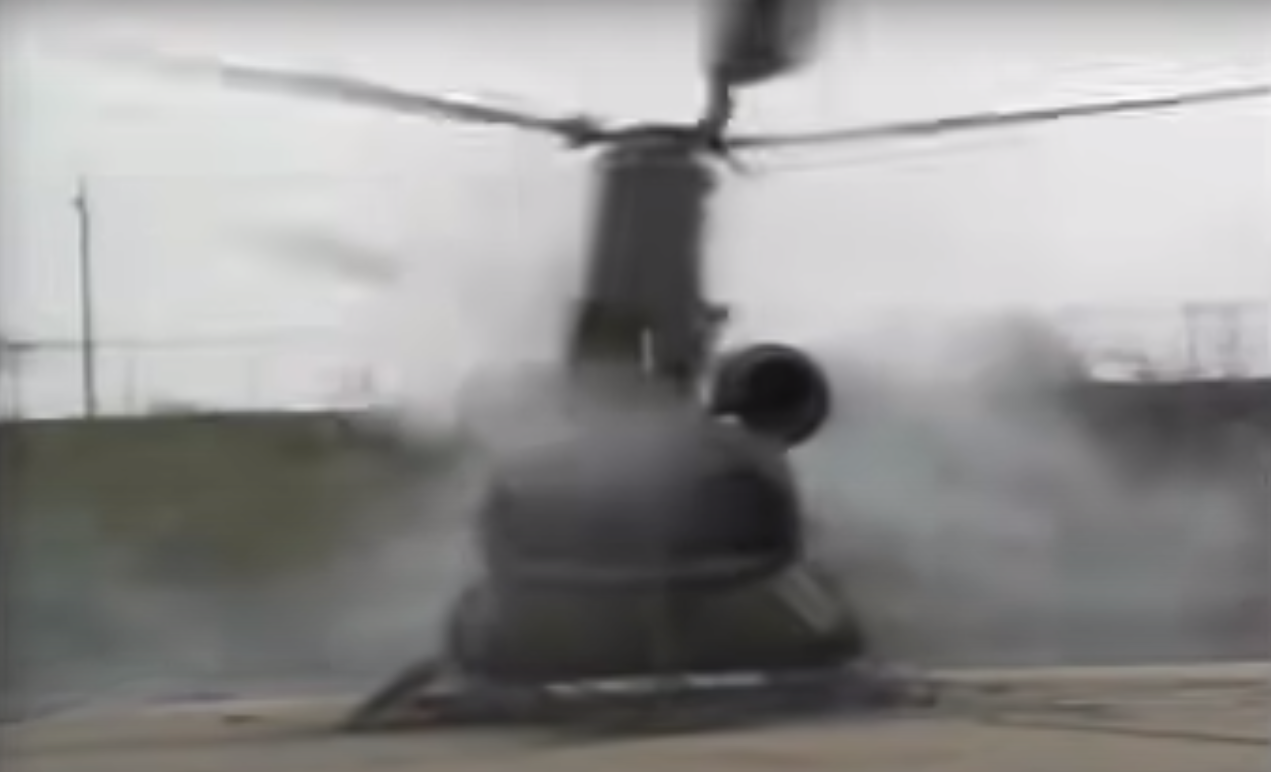
\includegraphics[width=\linewidth]{gambar/gr_3.png}
		\caption{}
		\label{fig:gr_3}
	\end{subfigure}
	\centering
	\begin{subfigure}{0.4\textwidth}
		\centering
		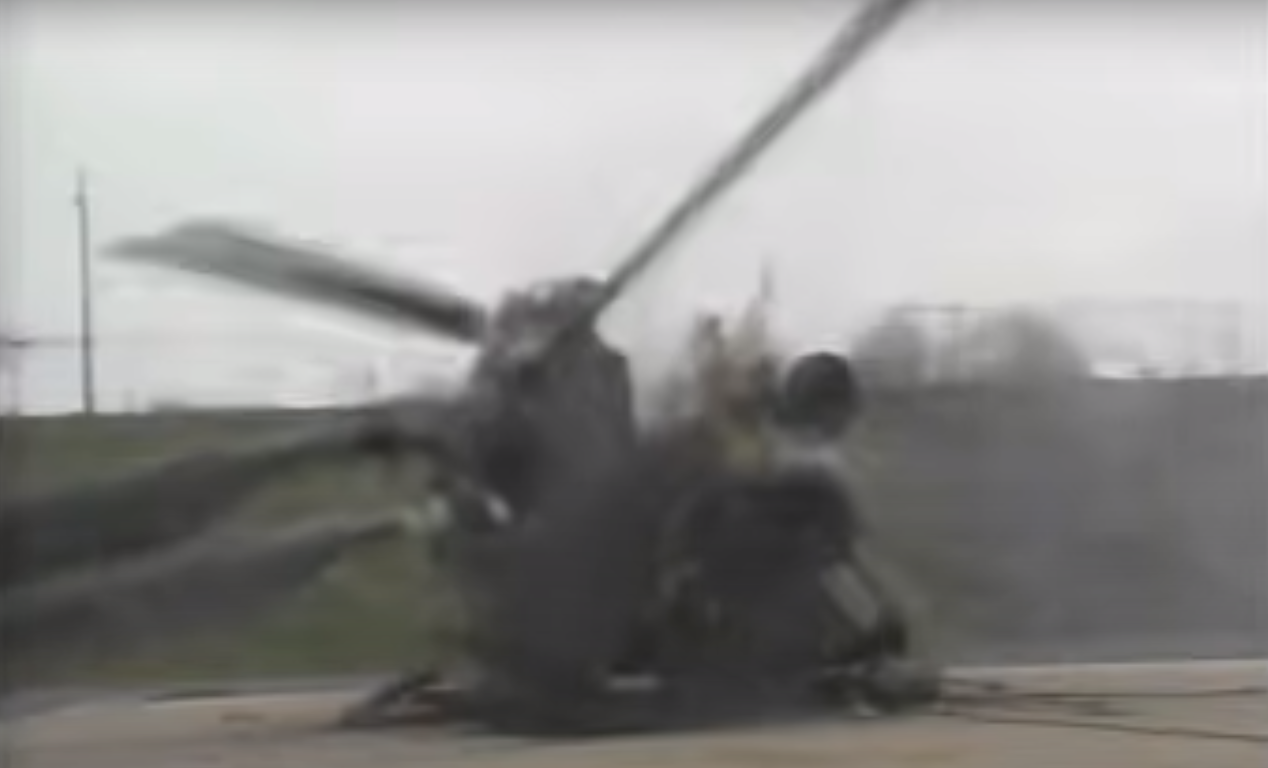
\includegraphics[width=\linewidth]{gambar/gr_4.png}
		\caption{}
		\label{fig:gr_4}
	\end{subfigure}
		\caption{(a) Kondisi saat helikopter stabil.(b) Sudah mulai terdapat getaran pada bagian kerangka helikopter (indikasi mulai terjadinya \textit{ground resonance}). (c) Terjadinya \textit{ground resonance} yang merusak bagian pada badan helikopter. (d) Pasca terjadinya \textit{ground resonance} pada helikopter.\\
		\urlstyle{rm}
		sumber: \url{https://www.youtube.com/watch?v=D2tHA7KmRME&t=3s}.}
		\label{fig:gr}
\end{figure}

Pada gambar \ref{fig:gr} menunjukkan situasi saat gerakan stabil \textit{lead/lag} tidak dapat mengkompensasi gerakan berlebih dalam bidang helikopter terhadap bilah rotor. Pusat gravitasi dari bilah rotor juga tidak lagi sejajar dengan penghubung pada rotor. Sehingga hal ini sangat berbahaya ketika helikopter bersentuhan dengan tanah. Posisi pusat gravitasi rotor yang tidak sejajar dengan penghubung rotor menghasilkan gaya sentrifugal yang tidak seimbang pada frekuensi tertentu \cite{Eckert2007AnalyticalAA}. Gaya tersebut menghasilkan gaya inersia periodik yang membuat seluruh badan helikopter bergetar terutama pada bagian pendaratannya ('\textit{chassis}' \textit{mode}). Jika salah satu frekuensi gaya inersia tersebut bertepatan dengan frekuensi pada '\textit{chassis}' \textit{mode} maka potensi terjadinya \textit{ground resonance} akan semakin besar \cite{bramwell2001bramwell}.

\begin{figure}[H]
	\centering
	\includegraphics[width=0.8\linewidth]{gambar/southwell_diagram.png}
	\caption{Diagram frekuensi \textit{chassis} dan rotor pada sistem \textit{fully articulated rotor} dengan sistem \textit{uncoupled}\cite{bramwell2001bramwell}.}
	\label{fig:southwell_diagram}
\end{figure}

Frekuensi yang dapat menyebabkan terjadinya fenomena \textit{ground resonance} dapat direpresentasikan dalam bentuk diagram seperti pada gambar \ref{fig:southwell_diagram}. Pada gambar tersebut, titik A merupakan frekuensi rotor saat \textit{hub} (penghubung) berada kondisi stasioner dan memiliki frekuensi yang lebih tinggi daripada frekuensi \textit{chassis mode} (garis putus-putus). 

Saat sistem \textit{uncoupled} mengacu pada kondisi saat gerakan pada rotor dan \textit{fuselage} dapat diperlakukan secara independen, tanpa ada pengaruh timbal balik yang signifikan. Sedangkan pada kondisi sebenarnya, helikopter memiliki sistem yang saling berhubungan satu sama lain, terutama antara sistem mekanik dan aerodinamik terhadap rotor dan \textit{fuselage}. Kondisi saling terhubung ini diakibatkan oleh perpindahan beban, getaran, dan energi antara kedua komponen tersebut. Ketika rotor menghasilkan gaya angkat atau berada pada kondisi \textit{idle}, maka hal tersebut akan menginduksi getaran dan gaya yang ditransimisikan ke badan helikopter \textit{fuselage}. 

Seiring dengan bertambahnya kecepatan pada rotor, frekuensi pada bilah rotor dan kecepatan pada rotor akan bertemu pada titik B dan C. Pada titik B, sistem masih dalam kondisi stabil. Sedangkan kondisi \textit{ground resonance} akan terjadi saat berada pada titik perpotongan di C. Pada kondisi sebenarnya (\textit{coupled}) memberikan visualisasi yang berbeda terhadap diagram pada gambar \ref{fig:southwell_diagram}. Saat kondisi ketidakstabilan terjadi, garis \textit{regressive mode} akan bertemu di sekitar titik C (gambar \ref{fig:southwell_coupled_diagram}), dan akan menyatu menjadi suatu rentang frekuensi yang mengindikasikan ketidakstabilan pada helikopter. 

\begin{figure}[H]
	\centering
	\includegraphics[width=0.75\linewidth]{gambar/southwell_coupled_diagram.png}
	\caption{Diagram frekuensi \textit{chassis} dan rotor pada sistem \textit{fully articulated rotor} dengan sistem \textit{coupled}\cite{bramwell2001bramwell}.}
	\label{fig:southwell_coupled_diagram}
\end{figure}


\section{Perhitungan Model Matematis}

Untuk dapat melakukan pendekatan secara analitik seperti yang telah diteliti oleh B.Bergeot et al \cite{BERGEOT201672}, diperlukan suatu model mekanik dari helikopter dengan derajat kebebasan minimum yang berpotensi mengalami fenomena \textit{ground resonance}. Oleh karena itu, dibutuhkan minimalnya sebanyak 5 derajat kebebasan (\textit{degree of freedom}/DOF). Helikopter terdiri atas \textit{fuselage} yang memiliki 4 bilah rotor dengan kecepatan konstan sebesar $\Omega$.

\begin{figure}[H]
	\centering 
	\begin{subfigure}{0.5\textwidth}
		\centering
		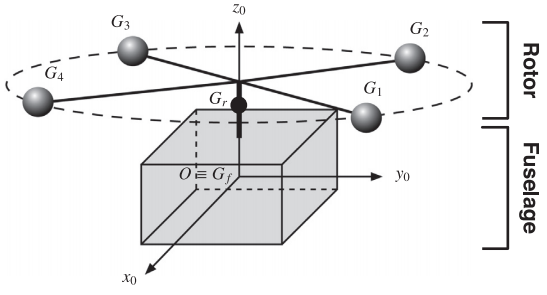
\includegraphics[width=\linewidth]{gambar/rotor_fuselage.png}
		\caption{}
		\label{fig:rotorfuselage}
	\end{subfigure}
	\centering
	\begin{subfigure}{0.35\textwidth}
		\centering
		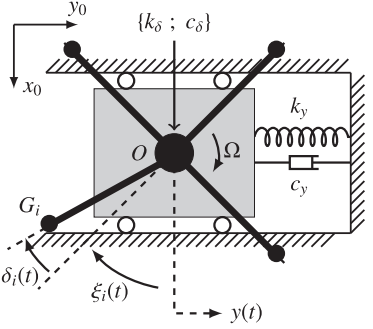
\includegraphics[width=\linewidth]{gambar/rotor_fuselage_topview.png}
		\caption{}
		\label{fig:topviewrotorfuslage}
	\end{subfigure}
	\caption{(a) Skema sederhana helikopter dengan 4 bilah rotor. (b) Skema helikopter dilihat dari atas \cite{BERGEOT201672}.}
	\label{fig:simplifiedmodel}
\end{figure}

Sistem koordinat kartesian digunakan dengan titik pusat di $O$. dengan $G_f$ merupakan pusat inersia \textit{fuselage} dan 3 sumbu kartesian pada sumbu-$x_0$, sumbu-$y_0$ dan sumbu-$z_0$ seperti yang terdapat pada gambar \ref{fig:rotorfuselage}. Kemudian terdapat $G_r$ yang merupakan pusat inersia rotor yang terletak di sumbu-$z_0$. Pada bagian \textit{fuselage} disederhanakan dengan representasi pemodelan yang tersusun seperti pada gambar \ref{fig:topviewrotorfuslage}, yaitu terdiri dari pegas, redaman dan massa dengan 1 arah translasi di sumbu-$y_0$. Selanjut pada arah translasi tersebut akan didefinisikan dalam domain waktu dengan koordinat $y(t)$. Pada masing-masing bilah rotor memiliki massa poin $G_i$ dengan [$i=1,2,3,4$], terletak pada jarak L dari sumbu-$z_0$. Sedangkan posisi pada bilah rotor ke-$i$ pada bidang-$x_0y_0$ sebagaimana persamaan \ref{eq:posisixy}.

\begin{equation}
\begin{cases}
x_{G_i} = L cos(\xi_i(t)+\delta_i(t))&(a) \\ 
y_{G_i} = y(t) + L sin(\xi_i(t)+\delta_i(t))&(b)
\end{cases}
\label{eq:posisixy}
\end{equation}

Dimana $\delta_i$ merupakan sudut \textit{lead/lag} pada bilah rotor ke-$i$. Sudut \textit{lead/lag} adalah perbedaan posisi bilah rotor saat waktu tertentu dengan posisi bilah rotor saat setimbangnya, yaitu $\xi_i(t)=\Omega t-(\pi/2)(i-1)$ sesuai pada gambar \ref{fig:topviewrotorfuslage}.

Persamaan gerak memiliki fungsi waktu untuk sistem 5 DOF pada helikopter, yaitu perpindahan \textit{fuselage} $y(t)$ dan 4 sudut \textit{lead/lag} $\delta_i(t)$. Kemudian pada tahap berikutnya adalah menurunkan persamaan gerak tersebut menggunakan metode Lagrange dengan variabel yang berkaitan ($T$=energi kinetik, $V$=energi potensial, dan $D$=disipasi energi Rayleigh) seperti pada persamaan \ref{eq:kinetik}, \ref{eq:potensial} dan \ref{eq:disipasi}.

\begin{align}
T &= \frac{1}{2}m_y\dot{y}^2 + \sum_{i=1}^{4}\frac{1}{2} m_{\delta} v^2_{\delta,i}
\label{eq:kinetik}
\\
V &= \frac{1}{2}k_yy^2+\sum_{i=1}^{4}\frac{1}{2}k_\delta \delta_i^2
\label{eq:potensial}
\\
D &= \frac{1}{2}c_y\dot{y}^2+\sum_{i=1}^{4}\frac{1}{2}c_\delta \dot{\delta}^2
\label{eq:disipasi}
\end{align}

Dengan bentuk umum persamaan dalam Lagrange seperti pada persamaan \ref{eq:lagrange_eq}.

\begin{align}
	\frac{d}{dt}\left(\frac{\partial T}{\partial \dot{q}_i}\right) - \frac{\partial T}{\partial q_i} + \frac{\partial D}{\partial \dot{q}_i} + \frac{\partial V}{\partial q_i} &= 0
	\label{eq:lagrange_eq}
\end{align}

Sehingga didapatkan:

\begin{equation}
	\begin{cases}
		(m_y+4m_\delta)\ddot{y}+c_y\dot{y}+k_yy+M_\delta\mathlarger{\sum}_{i=1}^{4}\left(\ddot{\delta_i}\cos(\xi_i+\delta_i)-(\Omega+\dot{\delta_i})^2\sin(\xi_i+\delta_i)\right) = 0 & (a) \\
		I_\delta\ddot{\delta_i}+c_\delta\dot{\delta_i}+k_\delta\delta_i+M_\delta \ddot{y}\cos(\xi_i+\delta_i)=0, \quad i=1,4 & (b)
	\end{cases}
	\label{eq:hasilmetodelagrang}
\end{equation}

Dengan ( $\dot{}$ ) merupakan tanda bahwa variabel tersebut telah diturunkan terhadap waktu $t$, $m_y$ merupakan massa \textit{fuselage}, $m_\delta$ adalah massa dari masing-masing bilah rotor. $M_\delta = m_\delta L$ dan $I_\delta = m_\delta L^2$ berturut-turut adalah momen statik dan momen inersia dari 1 bilah rotor. Subskrip $y$ adalah bagian dari \textit{fuselage} dan $\delta$ adalah bagian dari 1 buah bilah rotor. sehingga $c_y$ dan $c_\delta$ merupakan koefisien redaman dari \textit{fuselage} dan bilah rotor, $k_y$ dan $k_\delta$ adalah koefisien kekakuan linier dari \textit{fuselage} dan bilah rotor.

Untuk mendapatkan persamaan sistem yang \textit{time-invariant} (fungsi yang tidak bergantung mutlak pada waktu), maka persamaan \ref{eq:hasilmetodelagrang} harus dilinierisasi. Untuk itu, dilakukan asumsi bahwa sudut \textit{lead/lag} merupakan sudut yang sangat kecil ($\delta_i(t)<1$) kemudian menggunakan deret Taylor untuk mendapatkan sistem liniernya. Sehingga persamaan \ref{eq:hasilmetodelagrang} akan menjadi seperti persamaan \ref{eq:linearisasi_sudutkecil}.

\begin{equation}
	\begin{cases}
		(m_y+4m_\delta)\ddot{y}+c_y\dot{y}+k_yy+M_\delta\mathlarger{\sum}_{i=1}^{4}\left((\ddot{\delta}_i-\Omega^2\delta_i)\cos(\xi_i)-2\Omega \dot{\delta}_i\sin(\xi_i)\right) = 0 & (a) \\
		I_\delta\ddot{\delta}_i+c_\delta\dot{\delta}_i+k_\delta\delta_i+M_\delta \ddot{y}\cos(\xi_i)=0, \quad i=1,4 & (b)
	\end{cases}
\label{eq:linearisasi_sudutkecil}
\end{equation}

Transformasi Coleman melibatkan variabel yang mengubah gerakan masing-masing bilah rotor menjadi variabel gerakan kolektif. Untuk 4 bilah rotor akan terdapat 4 koordinat Coleman, diantaranya adalah $\delta_0$, $\delta_{1c}$, $\delta_{1s}$, dan $\delta_{cp}$ yang didefinisikan pada persamaan \ref{eq:colemantrans}.

\begin{equation}
\begin{aligned}
	\delta_0(t) &= \frac{1}{4}\mathlarger{\sum}_{i=1}^{4}\delta_i(t) && \text{(a)} \\
	\delta_{1c}(t) &= \frac{1}{2}\mathlarger{\sum}_{i=1}^{4}\delta_i(t) \cos(\xi_i(t)) && \text{(b)}\\
	\delta_{1s}(t) &= \frac{1}{2}\mathlarger{\sum}_{i=1}^{4}\delta_i(t) \sin(\xi_i(t)) && \text{(c)}\\
	\delta_{cp}(t) &= \frac{1}{4}\mathlarger{\sum}_{i=1}^{4}(-1)^i\delta_i(t) && \text{(d)}
\end{aligned}
\label{eq:colemantrans}
\end{equation}

Sebagaimana pada gambar \ref{fig:topviewrotorfuslage}, $\delta_i$ merupakan derajat kebebasan pada bilah rotor yang terlambat (\textit{lagging}), maka $\delta_0$ adalah \textit{lag} kolektif yang dimiliki rotor, sedangkan $\delta_{1c}$ dan $\delta_{1s}$ saling berhubungan dan merepresentasikan perpindahan dari pusat massa rotor $G_r$ pada bidangnya masing-masing di sumbu $x_0$ dan $y_0$ \cite{inproceedings}, sehingga didapatkan persamaan \ref{eq:pusatmassarotor}.

\begin{equation}
	\begin{cases}
		x_{G_r}(t) = -\mathlarger{\frac{L}{2}}\delta_{1s}(t)&(a) \\ 
		y_{G_r}(t) = \mathlarger{\frac{L}{2}}\delta_{1c}(t)&(b)
	\end{cases}
	\label{eq:pusatmassarotor}
\end{equation}

Dengan memasukkan variabel pada persamaan \ref{eq:colemantrans} ke persamaan \ref{eq:linearisasi_sudutkecil}, persamaan \ref{eq:linearisasi_sudutkecil}a dan \ref{eq:linearisasi_sudutkecil}b masing-masing akan persamaan \ref{eq:linearisasi}.

\begin{equation}
	\begin{cases}
	(m_y+4m_{\delta})\ddot{y}+c_y\dot{y}+k_yy+2M_{\delta}\ddot{\delta}_{1c}=0, &(a)\\
	I_{\delta}\ddot{\delta}_0+c_{\delta}\dot{\delta}_0+k_{\delta}\dot{\delta}_0=0&(b)\\
	I_{\delta}\ddot{\delta}_{1c}+c_{\delta}\dot{\delta}_{1c}+2I_{\delta}\Omega\dot{\delta}_{1s}+(k_{\delta}-I_{\delta}\Omega^2)\delta_{1c}+c_{\delta}\Omega\delta_{1s}+M_{\delta}\ddot{y}=0&(c)\\	I_{\delta}\ddot{\delta}_{1s}+c_{\delta}\dot{\delta}_{1s}-2I_{\delta}\Omega\dot{\delta}_{1c}+(k_{\delta}-I_{\delta}\Omega^2)\delta_{1s}-c_{\delta}\Omega\delta_{1c}=0&(d)\\
	I_{\delta}\ddot{\delta}_{cp}+c_{\delta}\dot{\delta}_{cp}+k_{\delta}\dot{\delta}_{cp}=0&(e)\\
	\end{cases}
	\label{eq:linearisasi}
\end{equation}

Pada persamaan \ref{eq:colemantrans} diatas, mode pada rotor hanya bergantung pada $\delta_{1c}$ dan $\delta_{1s}$, hal tersebut dikarenakan $\delta_{1c}$ dan $\delta_{1s}$ memengaruhi gaya dari rotor menuju ke \textit{fuselage}. Disisi lain, dari persamaan \ref{eq:linearisasi}, variabel $\delta_0$ dan $\delta_{cp}$ tidak saling berhubungan (\textit{uncoupled}) dan dapat diabaikan. Sehingga, hanya terdapat 3 derajat kebebasan dari pemodelan sederhana yang telah dilakukan diatas, yaitu $y$, $\delta_{1c}$, dan $\delta_{1s}$.

Persamaan gerak sederhana sesuai pada gambar \ref{fig:topviewrotorfuslage} dapat dituliskan dalam bentuk matriks pada persamaan \ref{eq:EOM}.

\begin{equation}
	\label{eq:EOM}
	\mathbf{M\ddot{X}}+(\mathbf{C}+\mathbf{G})\mathbf{\dot{X}}+\mathbf{KX}=\mathbf{0}
\end{equation}

Persamaan \ref{eq:linearisasi} dimuat dalam bentuk matriks dalam persamaan \ref{eq:EOM}. Dimana matriks $\mathbf{X}$, $\mathbf{M}$, $\mathbf{K}$, $\mathbf{C}$, dan $\mathbf{G}$ berturut-turut merupakan matriks derajat kebebasan, massa, kekakuan, redaman dan matriks giroskop dari sistem gerak. Masing-masing matriks tersebut didefinisikan pada persamaan \ref{eq:DOF} dan \ref{eq:matriks}.

\begin{equation}
	\label{eq:DOF}
	\mathbf{X}=[y \; \delta_{1c} \; \delta_{1s}]^t
\end{equation}

\begin{equation}
\begin{gathered}
	\mathbf{M}=\begin{bmatrix}
		1& \tilde{S}_d& 0\\
		\tilde{S}_c& 1& 0\\
		0& 0& 1
	\end{bmatrix}, \quad
	\mathbf{C}=\begin{bmatrix}
		\tilde{\lambda}_y& 0& 0\\
		0& \tilde{\lambda}_{\delta}& 0\\
		0& 0& \tilde{\lambda}_{\delta} 
	\end{bmatrix}, \\
	\mathbf{G}=\begin{bmatrix}
		0& 0& 0\\
		0& 0& 2\Omega\\
		0& -2\Omega& 0
	\end{bmatrix}, \
	\mathbf{K}=\begin{bmatrix}
		\omega^2_y& 0& 0\\
		0& \omega^2_{\delta}-\Omega^2& \tilde{\lambda}_{\delta}\Omega\\
		0& -\tilde{\lambda}_{\delta}\Omega& \omega^2_{\delta}-\Omega^2
	\end{bmatrix}
\end{gathered}
\label{eq:matriks}
\end{equation}

Dengan,

\begin{equation}
	\begin{gathered}
	\omega^2_y = \mathlarger{\frac{k_y}{(m_y+4m_{\delta})}},
	\quad 
	\omega^2_{\delta} = \mathlarger{\frac{k_{\delta}}{I_{\delta}}}, 
	\\
	\tilde{\lambda}_y = \mathlarger{\frac{c_y}{(m_y+4m_{\delta})}}, 
	\quad
	\tilde{\lambda}_{\delta} = \mathlarger{\frac{c_{\delta}}{I_{\delta}}}, 
	\\ 
	\tilde{S}_d = \mathlarger{\frac{2M_{\delta}}{(m_y+4m_{\delta})}}, 
	\quad 
	\tilde{S}_c = \mathlarger{\frac{M_{\delta}}{I_{\delta}}},
	\\
	I_{\delta} = m_{\delta}L^2, \quad M_{\delta}=m_{\delta}L
	\end{gathered}
\end{equation}

\textit{Ground resonance} berkaitan dengan analisis stabilitas pada persamaan \ref{eq:EOM}. Sehingga dapat didefinisikan dalam bentuk \textit{state-space}. Bentuk \textit{state-space} secara umum difenisikan pada persamaan \ref{eq:AdanQ}.

\begin{equation}
	\label{eq:AdanQ}
	\mathbf{\dot{Q}}=\mathbf{AQ}+\mathbf{BU}
\end{equation}

Dimana $\mathbf{\dot{Q}}$ adalah \textit{state vector} sebagai fungsi dari waktu, $\mathbf{A}$ dan $\mathbf{B}$ masing-masing adalah \textit{state matrix} dan \textit{input matrix} yang bernilai konstan. Sedangkan $\mathbf{U}$ adalah \textit{input} sebagai fungsi dari waktu. Karena pada persamaan \ref{eq:DOF} tidak memiliki \textit{input} maka persamaan dalam bentuk \textit{state-space} menjadi:

\begin{equation}
	\label{eq:state-space_simplified}
	\mathbf{\dot{Q}}=\mathbf{AQ}
\end{equation}

Dimana,

\begin{equation}
	\label{eq:state-space}
	\mathbf{Q}=[y \; \delta_{1c} \; \delta_{1s} \; \dot{y} \; \dot{\delta}_{1c} \; \dot{\delta}_{1s}]^t, \quad
	\mathbf{A}=\begin{bmatrix}
		\mathbf{0}& \mathbf{I}\\
		\mathbf{-M}^{-1}\mathbf{K}& \mathbf{-M}^{-1}(\mathbf{C}+\mathbf{G})
	\end{bmatrix}	
\end{equation}

Dengan $\mathbf{0}$ dan $\mathbf{I}$ masing-masing merupakan matriks bernilai $0$ dan matriks identitas berukuran 3x3. Solusi nilai eigen dan vektor eigen dari matriks $\mathbf{A}$ akan merepresentasikan fenomena dari \textit{ground resonance} melalui grafik imajiner terhadap kecepatan rotor $\Omega$ dan bagian riil terhadap kecepatan rotor $\Omega$.

\section{\textit{Logarithmic Decrement}}

Dalam suatu sistem periodik yang memiliki peredam. Pergerakan sistem tersebut seiring berjalannya waktu akan mengalami reduksi dan pada suatu waktu tertentu akan berhenti bergerak. Hal ini disebabkan oleh keberadaan peredam pada sistem. Penurunan amplitudo pada pergerakan suatu sistem yang teredam memiliki beberapa bentuk penurunan. Terdapat penurunan amplitudo yang terjadi secara linier dan logaritmik. Untuk penurunan yang bersifat logaritmik, terdapat peredam histeresis dan peredam viskositas. Pada bagian helikopter, peredam terdapat di bagian peredam hidrolik. Oleh karena itu, untuk analisis \textit{logarithmic decrement} pada helikopter digunakan peredam viskositas.

Dalam peredam viskositas, redaman terhadap penurunan amplitudo sistem terbagi menjadi 3 bentuk redaman, \textit{overdamped, critically damped,} dan \textit{underdamped}. Gambar \ref{fig:damping_motion} dan \ref{fig:underdamped} merupakan grafik yang menunjukkan gerakan penurunan amplitudo pada peredam viskositas. 

\begin{figure}[H]
	\centering
	\includegraphics[width=0.65\linewidth]{gambar/damping_motion.png}
	\caption{Gerakan pada sistem periodik pada peredam viskositas yang berbeda-beda \cite{rao2004mechanical}.}
	\label{fig:damping_motion}
\end{figure}

Penurunan secara logaritmik atau \textit{logarithmic decrement} merupakan paremeter spesifik yang dimiliki saat kondisi peredam viskositas berupa \textit{underdamped}. \textit{Logarithmic decrement} pada dasarnya juga merupakan parameter spesifik yang digunakan untuk menghitung koefisien redaman dari sistem liner \cite{Lojewski2020InfluenceOC}. 

\begin{figure}[H]
	\centering
	\includegraphics[width=0.7\linewidth]{gambar/underdamped.png}
	\caption{Grafik \textit{underdamped}.}
	\label{fig:underdamped}
\end{figure}

Persamaan \ref{eq:logdec} merupakan formulasi \textit{logarithmic decrement} pada kondisi \textit{underdamped}:

\begin{align}
	\delta = \frac{1}{m}ln\frac{x_1}{x_{m+1}}
	\label{eq:logdec}
\end{align}

Kemudian dari formulasi pada \ref{eq:logdec} dapat diformulasikan \textit{damping ratio} yang pada tahap berikutnya akan digunakan untuk pengolahan data pada helikopter.

\begin{align}
	\zeta=\frac{\delta}{\sqrt{\left( 2\pi \right)^2+\delta^2}}
\end{align}


\section{\textit{Finite Element Method}}

Metode elemen berhingga atau \textit{finite element method} merupakan sebuah metode numerik yang digunakan untuk mencari solusi dari mekanika kompleks serta permasalahan getaran dari suatu struktur. Pada metode ini, struktur asli pada objek dibagi menjadi elemen yang lebih kecil. Pada masing-masing elemen diasumsikan memiliki perilaku seperti bagian kontinu dari struktur yang disebut dengan elemen hingga (\textit{finite element}). Pada masing-masing elemen dihubungkan dengan suatu penghubung yang disebut dengan \textit{nodes} \cite{Lojewski2020InfluenceOC}.

Beberapa percobaan menggunakan analisis \textit{finite element} bertujuan untuk mendesain ulang dengan mengetahui terlebih dahulu deformasi yang terjadi pada suatu struktur, seperti yang dikejakan pada \cite{Gorecki2013}. Pada penelitian tersebut, dilakukan sebuah pemodelan pada helikopter menggunakan elemen stik model sebagai representasi bentuk simulasi pada pengujian resonansi sebenarnya dan langkah pertama untuk mengubah desain pada rotor helikopter. Gambar \ref{fig:ex_finite_element} merupakan contoh luaran yang didapatkan pada \cite{Gorecki2013}.

\begin{figure}[H]
	\centering
	\includegraphics[width=0.65\linewidth]{gambar/ex_finite_element.png}
	\caption{Salah satu contoh luaran pada \cite{Gorecki2013} untuk mencari deformasi dari simulasi pemodelan \textit{finite element}.}
	\label{fig:ex_finite_element}
\end{figure}

Pada gambar \ref{fig:ex_finite_element} merupakan salah satu contoh analisis menggunakan elemen hingga. Secara matematis, deformasi atau perpindahan secara transversal pada suatu elemen tertentu dapat diekspresikan dalam persamaan \ref{eq:FEM}.

\begin{align}
	\label{eq:FEM}
	w(x,y,t)=\sum_{i=1}^{n}N_i(x,y)w_i(t)
\end{align}

$N_i(x,y)$ merupakan \textit{shape function} yang berkorelasi dengan perpindahan pada \textit{nodes} $w_i(t)$ dan n merupakan penghubung ke-n. Jika diberikan gaya dari luar sebesar $f(x,y,t)$ pada elemennya. Maka gaya tersebut memiliki ekivalensi dengan bentuk $f_i(t)(i=1, 2, ...., n)$. Kemudian dapat didefinisikan dari energi kinetik serta potensial dari masing-masing elemen dalam bentuk matriks vektor ${\overrightarrow{\textbf{W}}}$. 

\begin{align}
	T=\frac{1}{2}\dot{\overrightarrow{\textbf{W}^T}}[m]\dot{\overrightarrow{\textbf{W}}}
	\label{eq:kinetik_FEM}
\end{align}

\begin{align}
	V=\frac{1}{2}\overrightarrow{\textbf{W}^T}[k]\overrightarrow{\textbf{W}}
	\label{eq:potensial_FEM}
\end{align}

dengan,

\begin{align*}
\overrightarrow{\textbf{W}}=\left\{ \begin{matrix} w_1(t) \\ w_2(t) \\ w_3(t) \\ .\\ .\\ .\\ w_n(t) \end{matrix}\right\}, \dot{\overrightarrow{\textbf{W}}}=\left\{ \begin{matrix} \dot{w}_1(t) \\ \dot{w}_2(t) \\ \dot{w}_3(t) \\ .\\ .\\ .\\ \dot{w}_n(t) \end{matrix}\right\}=\left\{ \begin{matrix} dw_1/dt \\ dw_2/dt \\ dw_3/dt \\ .\\ .\\ .\\ dw_n/dt \end{matrix}\right\}
\end{align*}

Dimana [m] dan [k] merupakan matriks massa dan kekakuan dari elemen. Apabila pada persamaan \ref{eq:kinetik_FEM} dan \ref{eq:potensial_FEM} disubtitusikan dengan menggunakan persamaan Lagrange \ref{eq:lagrange_eq}. Maka persamaan tersebut akan menjadi:

\begin{align}
	[m]\ddot{\overrightarrow{\textbf{W}}}+[k]\overrightarrow{\textbf{W}}=\overrightarrow{f}
	\label{eq:kinetik+potensial_lagrange}
\end{align}

$\overrightarrow{f}$ merupakan vektor gaya pada penghubung dan $\ddot{\overrightarrow{\textbf{W}}}$ merupakan percepatan pada \textit{nodes}. Dengan $\ddot{\overrightarrow{\textbf{W}}}$ merupakan turunan dari $\dot{\overrightarrow{\textbf{W}}}$ \cite{rao2004mechanical}. Semua proses matematis ini akan diproses menggunakan komputasi yang dimiliki oleh \textit{software} FEMAP dalam mencari penyelesaian serta memberikan representasi gerakan \textit{mode shape} pada helikopter yang akan dimodelkan.

\section{\textit{Ground Vibration Test} (GVT)}
\label{sec:GVT}

\begin{figure}[H]
	\centering
	\includegraphics[width=0.6\linewidth]{gambar/Eksiter_landing.png}
	\caption{Sumber penggetar pada bagian pendaratan \textit{aircraft} \cite{lubrina:hal-01059708}.}
	\label{fig:shaker_landing}
\end{figure}

\begin{figure}[H]
	\centering
	\includegraphics[width=0.6\linewidth]{gambar/Shaker_mainrotor.png}
	\caption{Penempatan \textit{shaker} pada bagian rotor utama \cite{Ciavarella2018AnEH}.}
	\label{fig:shaker_rotor}
\end{figure}

\textit{Ground Vibration Test} (GVT) memiliki tujuan utama untuk memberikan informasi mengenai karakterisasi struktur objek \textit{aircraft}. Dengan GVT dapat dilakukan identifikasi terhadap parameter modal eksperimental seperti frekuensi eigen, mode eigen, rasio redaman, massa umum, dan fungsi transfer yang menggambarkan perilaku dinamis struktural dari \textit{aircraft} yang diuji. Selain didapatkannya informasi tentang dinamika struktural \textit{aircraft}, juga akan didapatkan informasi fundamental untuk memvalidasi serta model terbaru dari \textit{Finite Element} (FE) dinamis \cite{Ciavarella2018AnEH}.

Untuk mendapatkan kualitas pengujian data yang baik, diperlukan pemahaman tentang struktur \textit{rotorcraft} serta persiapan yang tepat dalam melakukan GVT \cite{Ciavarella2018AnEH}. Selain itu, diperlukan juga peralatan yang memadai untuk memberikan \textit{input} getaran dalam mengukur respon getaran. Dengan ukuran dan berat yang cukup besar, rentang frekuensi yang dianalisis umum berada pada frekuensi rendah. Berdasarkan apa yang telah dikerjakan pada \cite{lubrina:hal-01059708} (contoh peletakan ada pada gambar \ref{fig:shaker_landing}) dilakukan analisis pada rentang frekuensi yang tidak lebih tinggi dari 50Hz. Batas frekuensi rendah dari rentang frekuensi bergantung pada karakteristik suspensi. Sedangkan pengukuran untuk melakukan identifikasi frekuensi eigen pada \textit{rigid body} batas frekuensi terendahnya tidak lebih kecil dari 1Hz. Sehingga sumber penggetar (\textit{shaker}) harus memiliki eksitasi hetaran pada frekuensi eigen yang rendah dengan kekuatan yang cukup \cite{lubrina:hal-01059708}. Disisi lain pada penelitian \cite{Ciavarella2018AnEH} memberikan 4 \textit{shaker} pada bagian rotor utama helikopter dengan arah lateral dan vertikal yang berkisar pada rentang 220 hingga 2200N (gambar \ref{fig:shaker_rotor}).

Untuk tujuan mitigasi, dilakukan 2 pengukuran gaya eksitasi dengan prinsip pengukuran yang berbeda. Pertama, gaya eksitasi diukur menggunakan alat ukur piezo elektrik. Kedua, gaya eksitasi diukur menggunakan arus koil yang disediakan oleh \textit{power amplifier} pada \textit{shaker}. Sensor perpindahan digunakan untuk mengukur perpindahan relatif dari armatur \textit{shaker} pada tempat peletakan \textit{shaker}. Sedangkan untuk mengukur respon vibrasi secara utama menggunakan akselerometer dalam pengukurannya. Pada penelitian \cite{lubrina:hal-01059708} digunakan sebanyak 500 sensor akselerometer untuk melakukan GVT, kemudian data hasil sensor diakuisisi menggunakan \textit{multichannel dynamic data} dari LMS Scadas III unutk selanjutnya diatur dengan perangkat lunak seperti Test.Lab \textit{software}.


\section{AS 565 MBe Panther}
\label{sec:AS565MBe}

\begin{figure}[H]
	\centering
	\includegraphics[width=0.6\linewidth]{gambar/AS565pic.png}
	\caption{Potret AS 565 MBe Panther saat mengudara.}
	\label{fig:AS565pic}
\end{figure}

AS 565 MBe Panther seperti pada gambar \ref{fig:AS565pic} adalah versi militer dari Eurocopter AS 365 Dauphin helikopter dengan mesin ganda dan bobot menengah yang multiguna. Helikopter ini dapat digunakan untuk berbagai peran militer, termasuk serangan tempur, dukungan tembakan, perang anti-kapal selam, perang anti-permukaan, pencarian dan penyelamatan, dan evakuasi medis \cite{AS565MBe}. Helikopter AS 565 MBe Panther dapat dimodifikasi sedemikian rupa untuk selanjutnya ditambahkan fitur persenjataan yang dapat mendukung kinerja helikopter ini dalam melakukan tugasnya. \textit{Profile} mengenai helikopter AS 565 MBe Panther dapat dilihat pada gambar \ref{fig:AS565MBe}. Dari informasi tersebut, helikopter ini memiliki berat maksimum agar helikopter dapat terbang adalah sebesar 4500kg. Sehingga, apabila modifikasi yang dilakukan pada helikopter merupakan modifikasi penambahan massa tanpa adanya modifikasi pada rotor, maka massa 4500kg akan menjadi batas maksimum modifikasi tersebut. Adapun potret dan dimensi spesifik terkait helikopter AS 565 MBe Panther dapat dilihat pada gambar \ref{fig:AS565MBe}, \ref{fig:as565mbe_atas}, \ref{fig:as565mbe_depan} dan \ref{fig:as565mbe_samping}.

\begin{figure}[H]
	\centering
	\includegraphics[width=0.7\linewidth]{gambar/Propertis_AS565MBe.png}
	\caption{\textit{Profile} helikopter AS 565 MBe Panther.}
	\label{fig:AS565MBe}
\end{figure}

\begin{figure}[H]
	\centering
	\includegraphics[width=0.9\linewidth]{gambar/as565_samping.png}
	\caption{Dimensi Helikopter AS 565 MBe Panther tampak samping.}
	\label{fig:as565mbe_samping}
\end{figure}

\begin{figure}[H]
	\centering
	\includegraphics[width=0.9\linewidth]{gambar/as565_atas.png}
	\caption{Dimensi Helikopter AS 565 MBe Panther tampak atas.}
	\label{fig:as565mbe_atas}
\end{figure}

\begin{figure}[H]
	\centering
	\includegraphics[width=0.7\linewidth]{gambar/as565_depan.png}
	\caption{Dimensi Helikopter AS 565 MBe Panther tampak depan.}
	\label{fig:as565mbe_depan}
\end{figure}